\documentclass[11pt,a4paper]{article}

\usepackage[a4paper, portrait, margin=1.1in]{geometry}
\usepackage[dvipsnames]{xcolor}
\usepackage[linktoc=none]{hyperref}
\hypersetup{
	colorlinks=true,
	linkcolor=blue,
	filecolor=magenta,      
	urlcolor=blue,
}

\usepackage{listings}
\usepackage{float}
\usepackage{graphicx}
\usepackage[justification=centering]{caption}
\usepackage{wrapfig}
\usepackage{amsmath}
\usepackage{xcolor}

\definecolor{codegreen}{rgb}{0,0.6,0}
\definecolor{codegray}{rgb}{0.5,0.5,0.5}
\definecolor{codepurple}{rgb}{0.58,0,0.82}
\definecolor{backcolour}{rgb}{0.95,0.95,0.92}
\definecolor{anti-flashwhite}{rgb}{0.95, 0.95, 0.96}


\renewcommand{\contentsname}{Indice}

\begin{document}

\begin{center}
	\Large{Corso di Laurea Magistrale in \\
	Artificial Intelligence and	Data Engineering}\\
	\vspace{0.2cm}
	\large{Seconda Relazione del Corso di Statistica II}\\
	\vspace{0.5cm}
	\Large\textbf{Prevedere quali squadre NBA parteciperanno ai playoff tramite metodi di Classificazione}\\
	\vspace{0.5cm}
	\large\emph{Edoardo Ruffoli}\\
	\vspace{0.5cm}
	\normalsize{9 Dicembre 2021}
\end{center}

\tableofcontents
\newpage
\section{Introduzione}
L'obiettivo dell'analisi è quello di realizzare e confrontare modelli di classificazione in grado di determinare se una squadra NBA possa qualificarsi ai Playoff a partire dalle statistiche di gioco registrate. 

Per quanto riguarda i contesti applicativi, un modello simile può essere utilizzato dalle agenzie di scommesse per il calcolo delle quote sportive oppure dalle franchigie NBA stesse per valutare se l'andamento corrente di una squadra possa consentire una qualificazione ai Playoff o meno.

\section{Dataset}
L'analisi è stata svolta facendo uso delle tabelle \emph{Teams General Traditional}, \emph{Teams General Advanced} e \emph{NBA Standings} reperibili sul sito ufficiale NBA che contengono le statistiche stagionali e le informazioni relative ai Playoff per ogni squadra:
\begin{center}
    \url{https://www.nba.com/stats/teams/traditional}\\
    \url{https://www.nba.com/stats/teams/advanced}\\
    \url{https://www.nba.com/standings}\\
\end{center}

Dal momento che non vi è un link per scaricare le sopracitate tabelle, è stato utilizzato uno script Python scaricabile al seguente \href{https://raw.githubusercontent.com/edoardoruffoli/Statistics/master/SecondProject/nba_stats_scraper_v2.py}{link} il cui funzionamento sarà analizzato nel dettaglio nell'appendice di questa relazione.

Per raggiungere una numerosità adeguata al metodo di analisi sono stati utilizzati i dati delle ultime 21 stagioni NBA: la scelta di includere osservazioni riguardanti le medesime squadre, registrate in anni differenti, non comporta il rischio di avere una ripetizione degli stessi andamenti. Da una stagione all'altra sono solite variare, talvolta anche radicalmente, la composizione ma soprattutto le prestazioni delle singole squadre. 

\subsection{Contenuto del Dataset}
La tabella contiene 42 colonne e 626 osservazioni. Ai fini dell'analisi sono state utilizzate le seguenti 12 colonne: 
\begin{itemize}
    \item \textbf{FGA}: numero di tiri tentati a partita (decimale positivo).
    \item \textbf{FG3A}: numero di tiri da tre punti tentati a partita (decimale positivo).
    \item \textbf{FTA}: numero di tiri liberi tentati a partita (decimale positivo).
    \item \textbf{REB}: numero di rimbalzi catturati a partita (decimale positivo).
    \item \textbf{AST}: numero di assist a partita (decimale positivo).
    \item \textbf{TOV}: numero di palle perse per partita (decimale positivo).
    \item \textbf{STL}: numero di palle recuperate per partita (decimale positivo).
    \item \textbf{BLK}: numero di stoppate a partita (decimale positivo).
    \item \textbf{PTS}: numero di punti segnati a partita (decimale positivo).
    \item \textbf{OFF\_RATING}: numero di punti segnati da una squadra per 100 possessi di gioco (decimale positivo).
    \item \textbf{DEF\_RATING}: numero di punti subiti da una squadra per 100 possessi di gioco (decimale positivo).
    \item \textbf{PLAYOFF}: indica se la squadra si sia qualificata ai Playoff (binario).
\end{itemize}

NB: Se fossero stati utilizzati i dati totali e non quelli per partita, il modello sarebbe stato utilizzabile solo al termine della stagione, perdendo quindi di utilità.

\subsection{Data Preprocessing}
Anche in questa analisi, è stato preferito eliminare le osservazioni relative a stagioni con un numero di partite giocate diverso da 82, soprattutto perché relative a stagioni fortemente influenzate da fattori esterni (ad esempio la pandemia di Covid 19). 
Il dataset passa quindi da 626 a 534 osservazioni.

La selezione dei fattori di ingresso è stata effettuata in modo da evitare ridondanza di informazioni tra colonne diverse.
Non è stato considerato come fattore di ingresso il numero di vittorie perché non è un dato esprimibile nella forma "per partita" ma solo totale, inoltre non sono stati considerati tutti i fattori espressi in valori percentuali o nominali.

\subsection{Considerazioni Preliminari}
Il dataset presenta 248 osservazioni relative a squadre che non si sono qualificate per i Playoff (PLAYOFF = 0), e 286 a squadre che si sono qualificate per i Playoff (PLAYOFF = 1): il dataset è dunque sostanzialmente bilanciato.

Dallo scatter plot, è possibile osservare una distinzione tra le due classi nei grafici riguardanti i parametri avanzati OFF\_RATING e DEF\_RATING che potrebbero rivelarsi i più significativi per una classificazione precisa. I grafici degli altri fattori di ingresso non presentano una distinzione evidente tra le due classi.
\begin{figure}[h]
    \hspace{-1.7cm}
	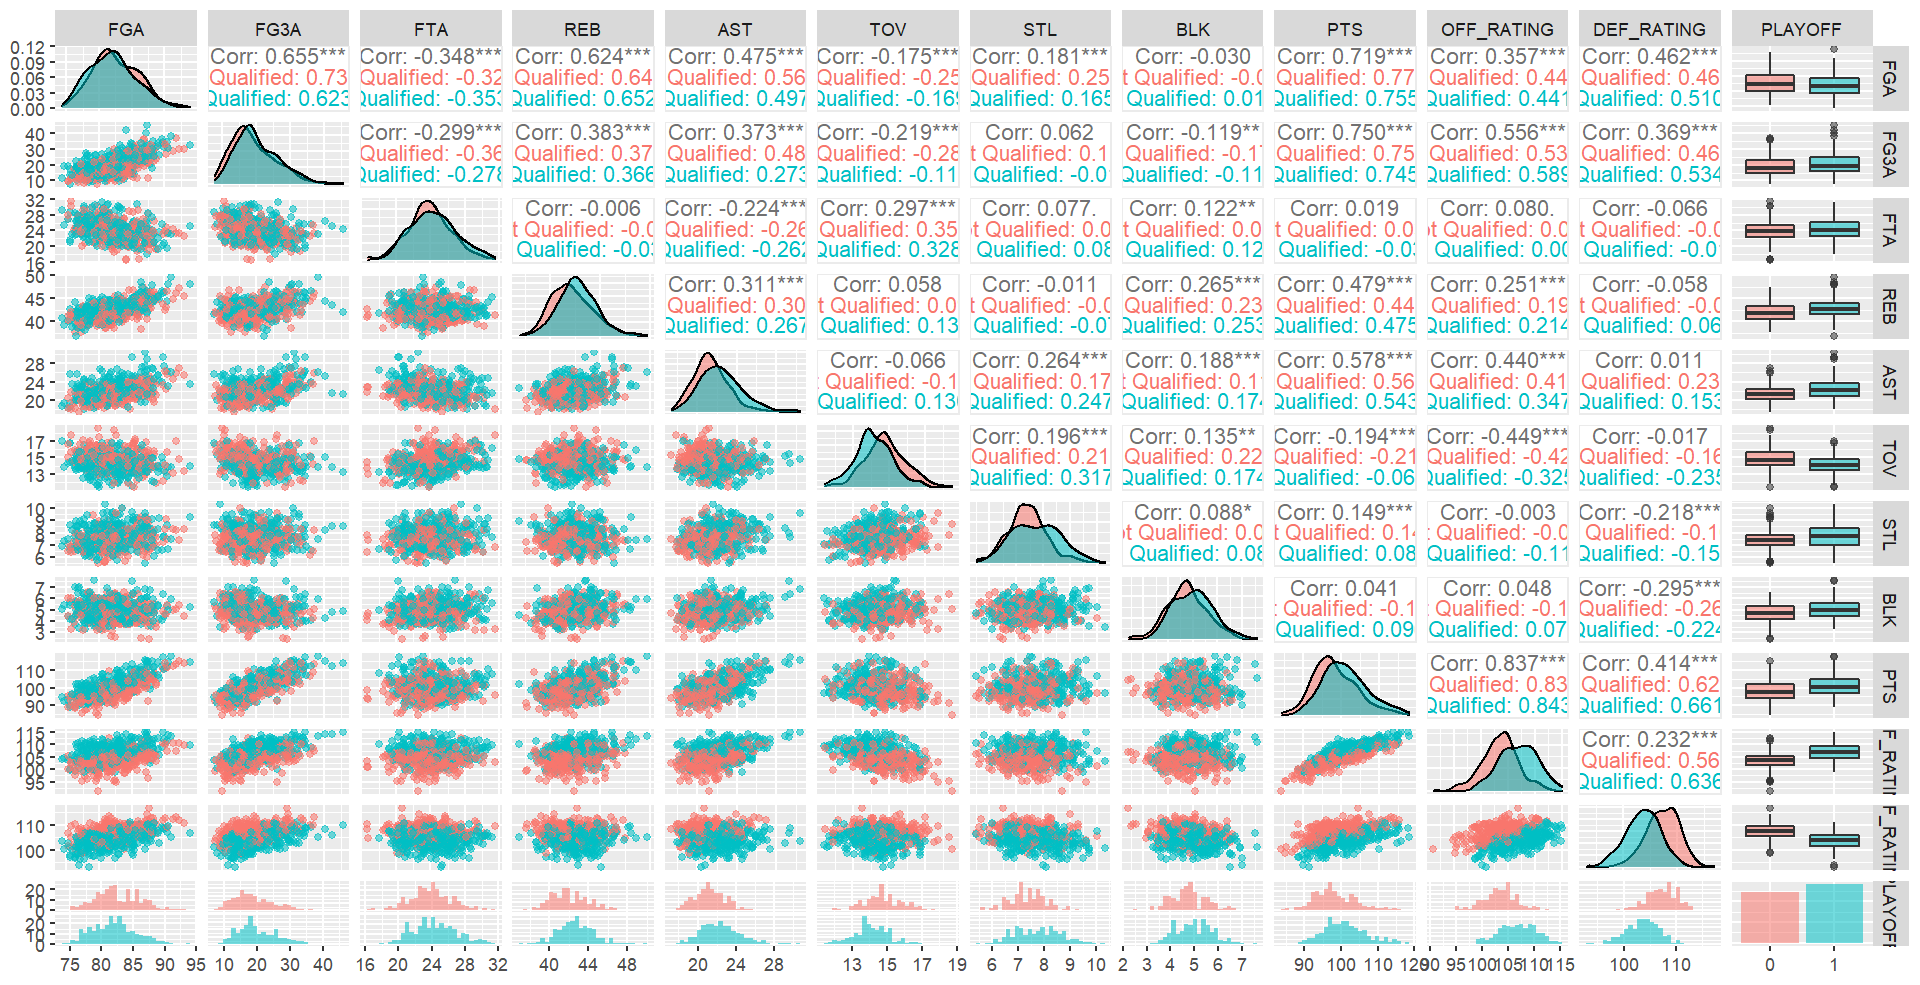
\includegraphics[scale=0.55]{imgs/scatter_plot.png}
    \end{figure}
\vspace{-0.4cm}

\newpage
\section{Analisi}
Dopo la preparazione dei dati, sono state analizzate le performance di tre modelli di classificazione: Discriminante Lineare, Discriminante Quadratico e Regressione Logistica.
Le accuratezze ottenute di seguito, sono state calcolate senza effettuare divisioni tra training set e test set e pertanto risultano leggermente superiori a quelle effettive.
Non è stato ritenuto necessario affiancare all'accuratezza altre metriche di valutazione come ad esempio Precision, Recall e F1 Score: il dataset in questione è bilanciato, e quindi l'accuratezza è una metrica sufficientemente affidabile per l'analisi.

\subsection{Classificazione mediante Analisi Discriminante Lineare}
L'analisi discriminante lineare (lda) restituisce un'accuratezza del 90\% classificando correttamente 485 osservazioni. La sensibilità ottenuta è circa 93\% e la specificità 88\%: non essendoci una differenza significativa tra i due valori, si può considerare la soglia di classificazione al 50\% adeguata per il problema.

\begin{lstlisting}[language=bash,basicstyle=\tiny,tabsize=2,frame = single]
Confusion Matrix
            actual 1 actual 0
predicted 1      266       29
predicted 0       20      219

Accuracy 0.9082397
\end{lstlisting}

\subsection{Classificazione mediante Analisi Discriminante Quadratica}
L'analisi discriminante quadratica (qda) restituisce un'accuratezza del 90\% classificando correttamente 482 osservazioni. Ancora una volta i valori simili di sensibilità (90\%) e specificità (90\%), confermano l'adeguatezza della soglia considerata.

\begin{lstlisting}[language=bash,basicstyle=\tiny,tabsize=2,frame = single]
Confusion Matrix
            actual 1 actual 0
predicted 1      259       25
predicted 0       27      223

Accuracy 0.9026217
\end{lstlisting}

\subsection{Classificazione mediante Regressione Logistica}
La regressione logistica (glm) restituisce un'accuratezza leggermente migliore dei due modelli precedenti, pari al 91\%, classificando correttamente 487 osservazioni. Le considerazioni su sensibilità e specificità sono analoghe ai casi precedenti.

\begin{lstlisting}[language=bash,basicstyle=\tiny,tabsize=2,frame = single]
Confusion Matrix
            actual 1 actual 0
predicted 1      265       26
predicted 0       21      222

Accuracy 0.911985
\end{lstlisting}

Come emerso dall'analisi preliminare dello scatter plot iniziale, i fattori di ingresso OFF\_RATING e DEF\_RATING, i due indicatori avanzati selezionati per l'analisi, risultano essere i predittori più significativi del modello regressivo. Osservando il grafico tra i due fattori di ingresso, si nota una divisione abbastanza netta tra le classi della classificazione.

\begin{figure}[h]
	\hspace{-2.30cm}
	\begin{minipage}{.57\textwidth} 
		\begin{lstlisting}[language=bash,basicstyle=\tiny,tabsize=2,frame = single]
> summary(data.glm)

Call:
glm(formula = PLAYOFF~., family = binomial, data = data)

Deviance Residuals: 
     Min        1Q    Median        3Q       Max  
-2.73115  -0.15262   0.01042   0.18257   2.47680  

Coefficients:
            Estimate Std. Error z value Pr(>|z|)    
(Intercept) 54.95567   18.22184   3.016  0.00256 ** 
FGA         -0.35002    0.20150  -1.737  0.08237 .  
FG3A         0.04882    0.05657   0.863  0.38809    
FTA          0.04430    0.11614   0.381  0.70287    
REB          0.02024    0.19672   0.103  0.91807    
AST          0.17054    0.14805   1.152  0.24936    
TOV         -0.65357    0.27830  -2.348  0.01885 *  
STL          0.43022    0.29679   1.450  0.14717    
BLK         -0.01243    0.26358  -0.047  0.96239    
PTS          0.23461    0.16863   1.391  0.16413    
OFF_RATING   0.75669    0.19003   3.982 6.84e-05 ***
DEF_RATING  -1.22743    0.15650  -7.843 4.40e-15 ***
        \end{lstlisting}
    \end{minipage}
	\begin{minipage}{0.5\textwidth} 
		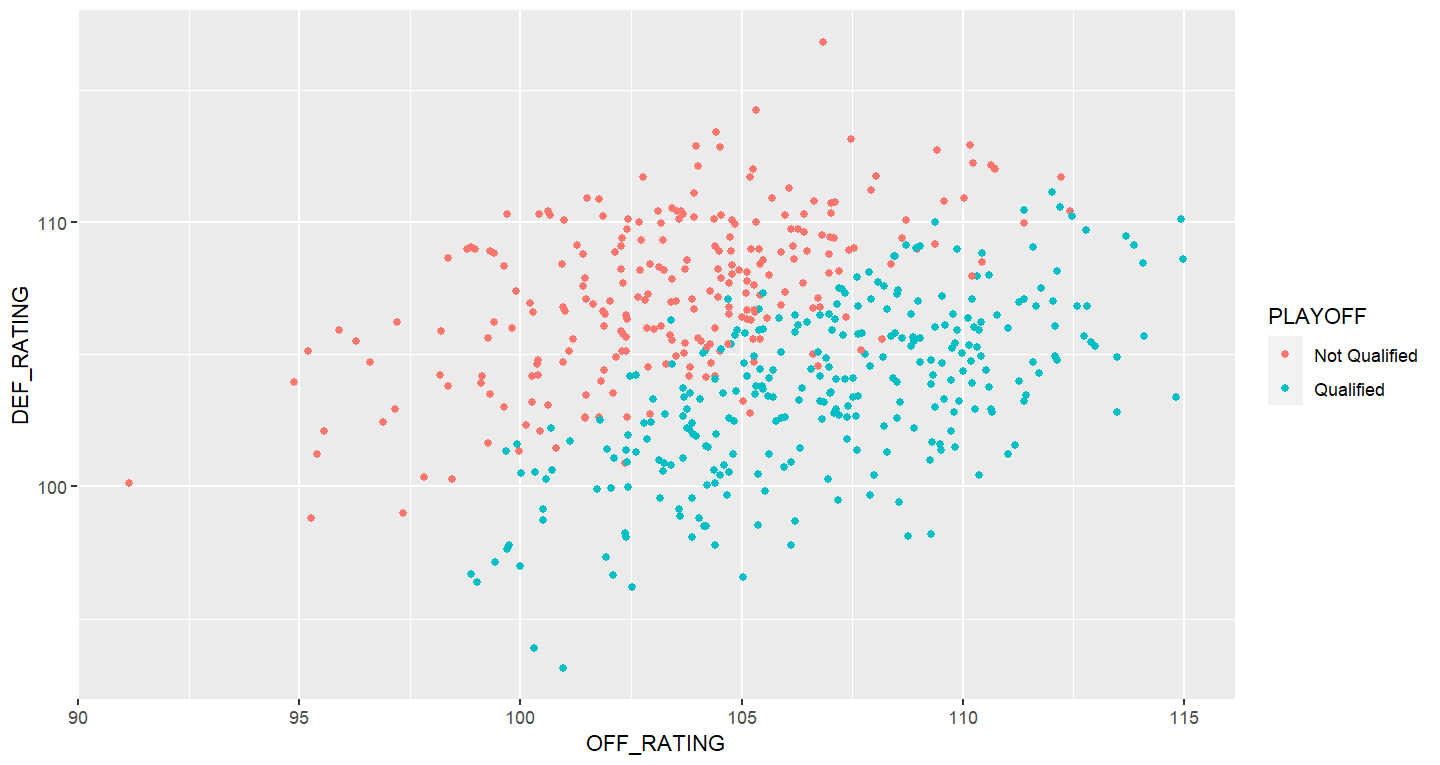
\includegraphics[scale=.45]{imgs/OFF_RATING-DEF_RATING_plot.png}
	\end{minipage}
\end{figure}
\newpage

\section{Confronto}
I modelli costruiti restituiscono risultati molto simili tra loro, risulta inevitabile quindi l'utilizzo di metodi di confronto più elaborati per stabilire quale sia il miglior classificatore.

\subsection{Confronto ROC}
Osservando il grafico delle curve ROC, non si notano sostanziali differenze tra i vari modelli. Andando a comparare i valori di AUC invece, il modello lineare presenta un valore leggermente inferiore agli altri due modelli.

\begin{figure}[h]
    \hspace{-1.7cm}
	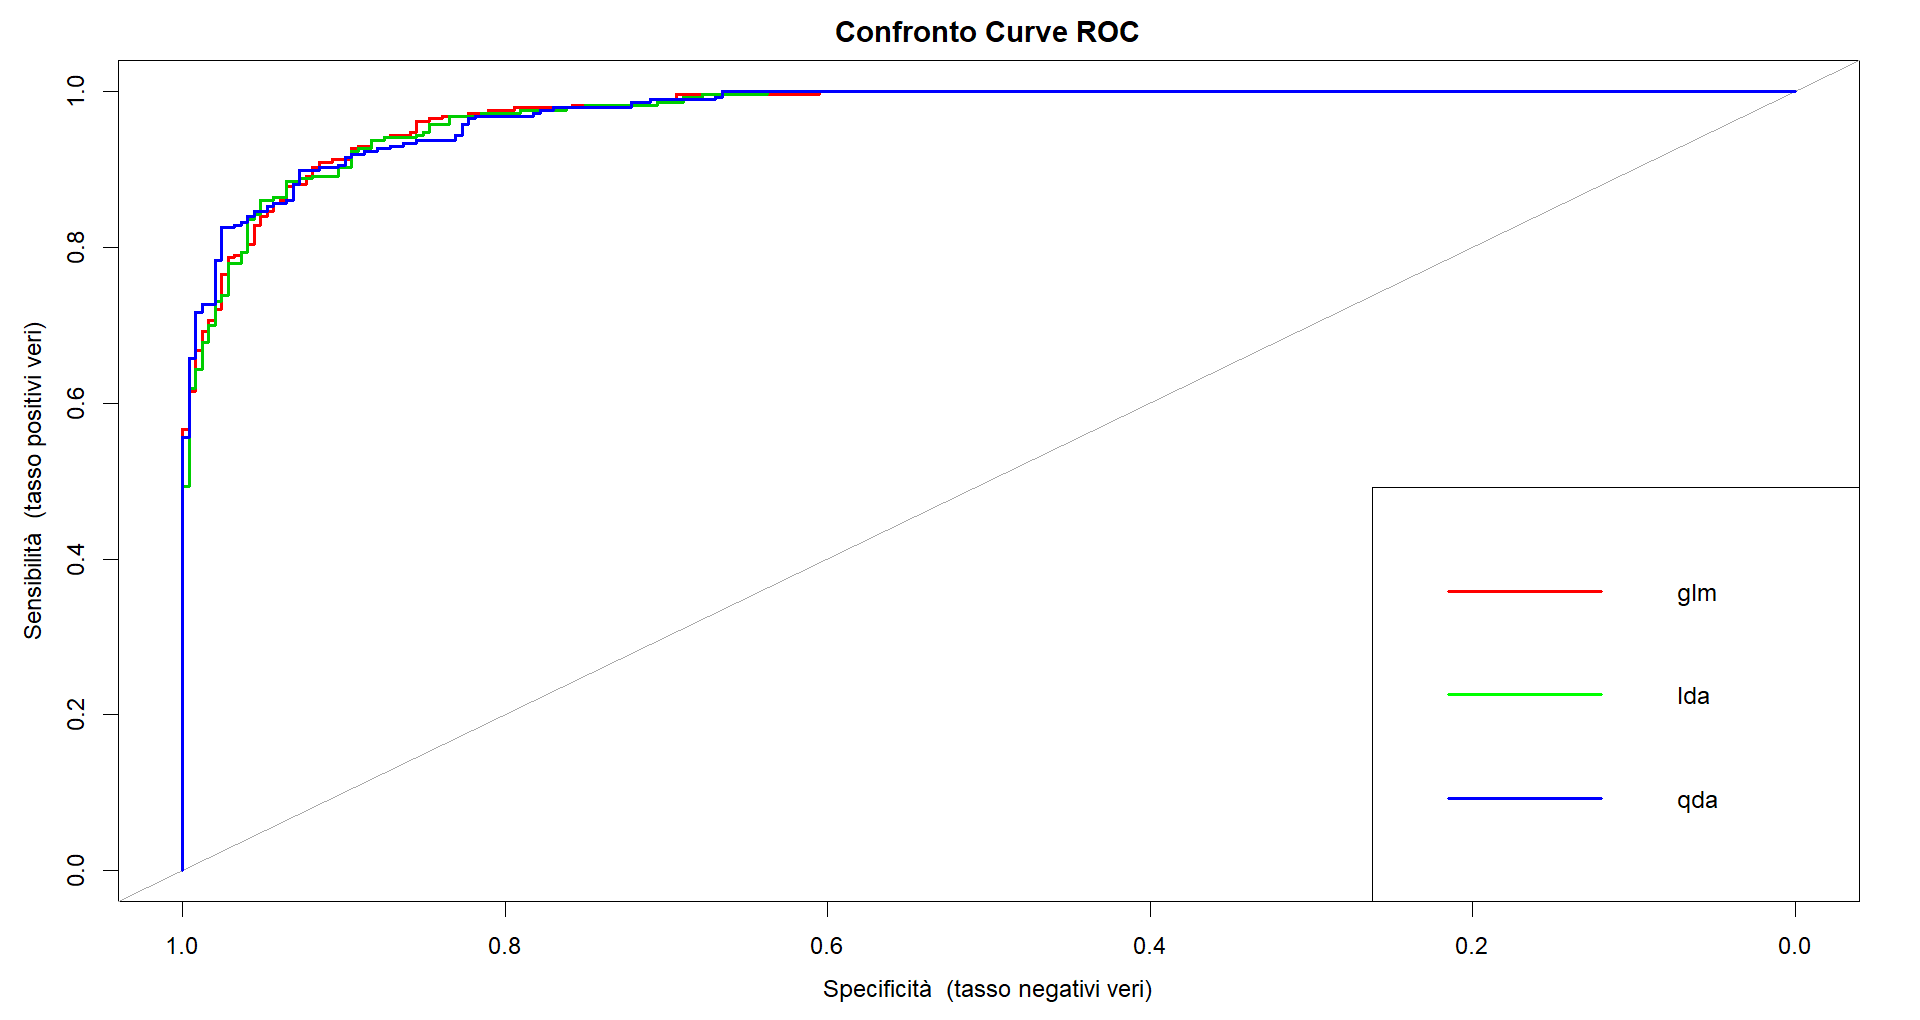
\includegraphics[scale=0.55]{imgs/roc_curves_comparison.png}
    \end{figure}
\vspace{-0.4cm}

\begin{lstlisting}[language=bash,basicstyle=\tiny,tabsize=2,frame = single]
> data.glm.roc$auc
Area under the curve: 0.9739
> data.lda.roc$auc
Area under the curve: 0.9728
> data.qda.roc$auc
Area under the curve: 0.9739
\end{lstlisting}

\subsection{Confronto Autovalutazione}
Per effettuare l'autovalutazione dei modelli, le 534 osservazioni del dataset sono state divise in un sottoinsieme di 100, utilizzate come \emph{test set}, e le restanti 434 sono state utilizzate come \emph{training set}. Tale procedimento è stato ripetuto per un totale di 100 iterazioni, per garantire rilevanza statistica.
Sono stati confrontati i valori medi e le deviazioni standard dell'accuratezza e dell'AUC ottenuti per ogni modello.

\begin{lstlisting}[language=bash,basicstyle=\tiny,tabsize=2,frame = single]
Results:
            mean(accuracy)  sd(accuracy)        mean(AUC)       sd(AUC)
lda         0.8994          0.0281346           0.967579        0.01401571
qda         0.8814          0.03253654          0.9592355       0.01628317
glm         0.8993          0.02815021          0.967579        0.01401571
\end{lstlisting}
\vspace{-0.5cm}
\begin{figure}[h]
	\hspace{-1.80cm}
	\begin{minipage}{.57\textwidth} 
	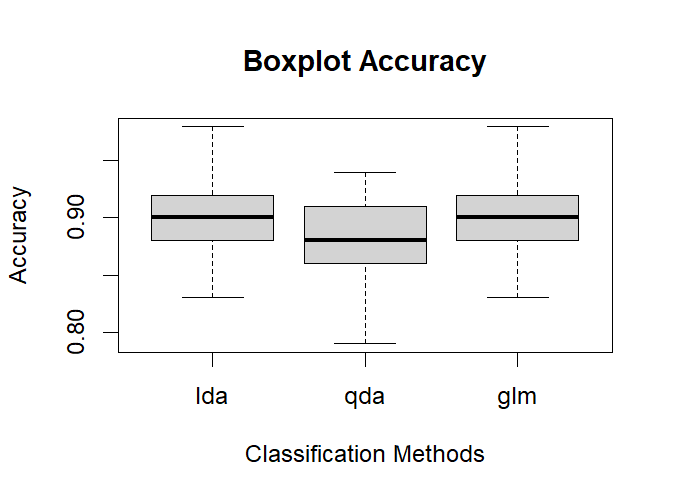
\includegraphics[scale=.8]{imgs/boxplot_accuracy.png}
    \end{minipage}
	\begin{minipage}{0.5\textwidth} 
		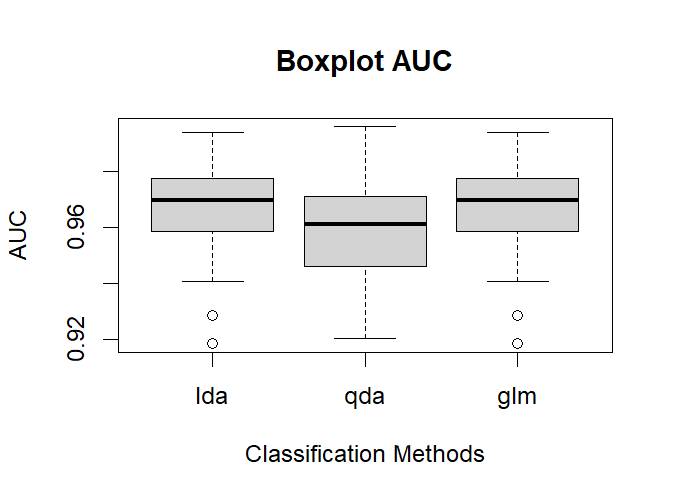
\includegraphics[scale=.8]{imgs/boxplot_AUC.png}
	\end{minipage}
\end{figure}

Come preannunciato, le accuratezze calano lievemente rispetto a quelle ottenute senza la divisione del dataset in training test e test set.
È interessante notare come il modello lda non abbia più il valore di AUC inferiore, come invece era emerso dal confronto delle curve ROC: è infatti il modello a discriminante quadratico che risulta essere il peggiore per entrambi i parametri considerati. 

Il modello a discriminante lineare e la regressione logistica presentano valori di accuratezza molto simili e ottengono sempre gli stessi valori di AUC, anche ripetendo il test con seed diversi.
Per questo motivo è stato ritenuto necessario effettuare un test per valutare se la lieve differenza di accuratezza sia o meno statisticamente significativa. È stato utilizzato il test Wilcoxon in quanto è un test non parametrico, dato che non abbiamo informazioni sulla distribuzione dell'accuratezza. Dato il valore estremamente elevato del p-value, che ci impedisce di rigettare l'ipotesi nulla, si può concludere che non vi sia differenza statistica tra le accuratezze registrate per i modelli lda e glm e che quindi i risultati forniti da essi siano statisticamente equivalenti. 

\begin{lstlisting}[language=bash,basicstyle=\tiny,tabsize=2,frame = single]
> wilcox.test(acc[,1], acc[,3])

	Wilcoxon rank sum test with continuity correction

data:  acc[, 1] and acc[, 3]
W = 500142, p-value = 0.9912
alternative hypothesis: true location shift is not equal to 0

\end{lstlisting}

\subsection{Confronto Robustezza}
L'ultimo test effettuato sui modelli è un test di robustezza. Ad ogni iterazione viene cambiata la classe di un'osservazione e viene eseguito un'autovalutazione dei modelli sul dataset modificato.
L'autovalutazione viene ripetuta solo 10 volte per iterazione per non appesantire eccessivamente la complessità.

Il modello a Discriminante Quadratico presenta un andamento più lineare e quindi sicuramente meno robusto  rispetto agli altri due modelli.
L'andamento dei modelli lda e glm rappresenta un'ulteriore conferma dell'equivalenza dei due modelli per l'analisi in questione.

\begin{figure}[h]
    \hspace{-.8cm}
	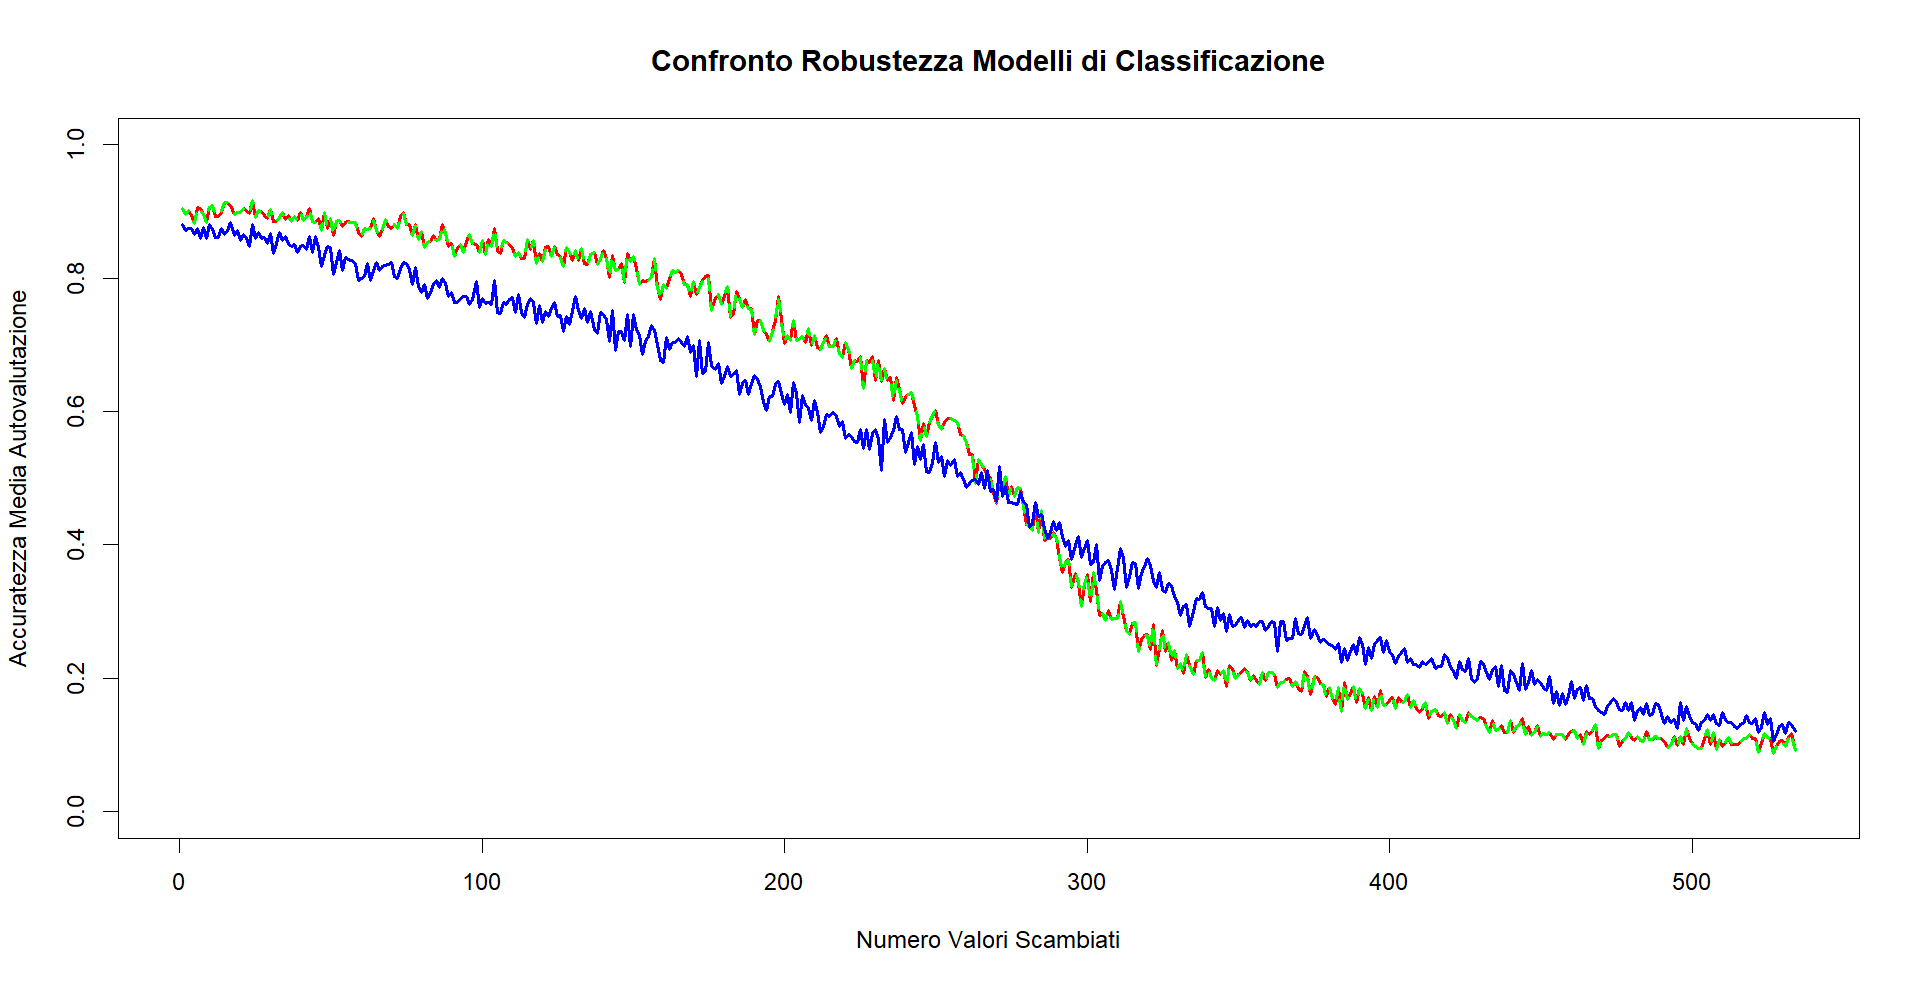
\includegraphics[scale=0.5]{imgs/robustness.png}
    \end{figure}
\vspace{-0.4cm}

\section{Conclusioni}
I vari test effettuati per confrontare i modelli hanno restituito esiti leggermente migliori per i modelli lda e glm, inoltre, tra i suddetti modelli, è stata registrata una forte somiglianza che non ha permesso di preferirne uno piuttosto che l'altro.

L'accuratezza ottenuta è soddisfacente e difficilmente migliorabile: non è stato possibile ottenere un'accuratezza più elevata sia costruendo i modelli tramite una riduzione di fattori, sia considerando combinazioni di fattori di ingresso differenti da quelli utilizzati, sia costruendo i modelli logaritmici (coerentemente con le conclusioni della prima relazione in quanto la natura dei dati analizzati è lineare).

\hspace{-0.7cm}
\vspace{0.1cm}
\begin{minipage}{0.5\textwidth} 
\vspace{0.1cm}
\setlength{\parindent}{1.5em}
\indent Un'ipotesi sull'impossibilità di incrementare l'accuratezza e sulla somiglianza tra i risultati ottenuti con i tre modelli analizzati è che essi presentino le stesse difficoltà a classificare le medesime osservazioni: quelle che sono "al confine" tra una zona e l'altra.
Risulta ben visibile osservando il partition plot di un modello a discriminante lineare su due fattori di ingresso (OFF\_RATING e DEF\_RATING, i più significativi). Gli errori, indicati in rosso, sono tutti a cavallo delle due partizioni.
\end{minipage}
\begin{minipage}{0.5\textwidth} 
    \hspace{0.5cm}
    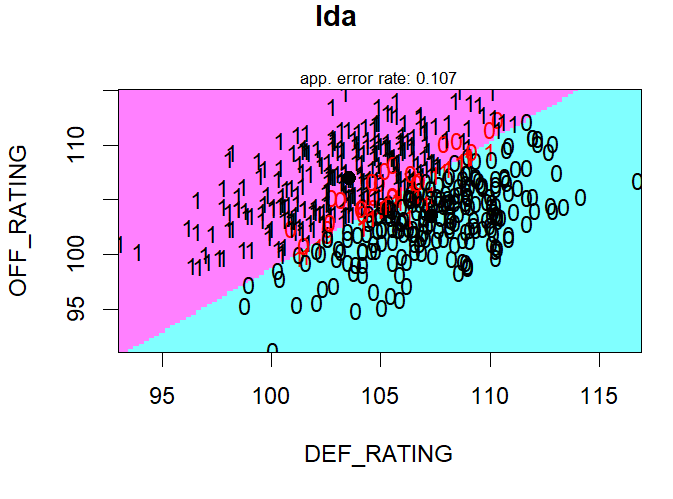
\includegraphics[scale=.6]{imgs/partition_plot_lda.png}
\end{minipage}

Ciò è dovuto in parte anche a un problema intrinseco dei dati stessi: nel campionato NBA, si qualificano ai Playoff le prime 8 squadre di ognuna delle due Conference, per percentuale di partite vinte. Perciò è possibile che una squadra con una W\_PCT più bassa riesca a qualificarsi ai Playoff e una squadra con una W\_PCT più alta, e quindi verosimilmente con statistiche migliori, no.

Una soluzione potrebbe essere quella di suddividere le osservazioni in base alla Conference, ottenendo quindi due tabelle.
Sarebbe possibile ottenere un'accuratezza migliore realizzando un modello di classificazione come sintesi tra il miglior modello ottenuto per ognuna delle due tabelle.

Per classificare un'osservazione sarà sufficiente utilizzare il modello ottenuto con i dati della Conference di appartenenza dell'osservazione; una soluzione simile richiede solamente che sia conosciuto un fattore di ingresso aggiuntivo, la Conference di appartenenza (che è ricavabile a costo zero, semplicemente conoscendo il nome di una squadra).

\newpage
\appendix
\section{Appendice}
 Lo script utilizzato per ottenere le due tabelle utilizzate nell'analisi, fa uso delle \emph{nba-api} ufficiali per Python, consultabili al seguente link \url{https://github.com/swar/nba_api}.
 
La funzione \emph{get\_data()}, per ogni stagione indicata nella lista "seasons", scarica i dati sotto forma di liste di \emph{dictonaries} utilizzando le funzione \emph{leaguedashteamstats\.LeagueDashTeamStats} e \emph{leaguestandings.LeagueStandings} delle \emph{nba-api}. Il fattore di ingresso \emph{PLAYOFF}, è stato ricavato sfruttando il campo \emph{PlayoffRank} che contiene il piazzamento di una squadra all'interno della propria conference. Si ricorda che partecipano ai Playoff NBA le prime 8 qualificate di ognuna delle due conference.
 
 \vspace{0.5cm}
 \begin{lstlisting}[language=python,tabsize=1,frame = single]
# 1 for teams that qualified for the playoff, 0 otherwise
l['PLAYOFF'] = 1 if playoff_rank <= 8 else 0
\end{lstlisting}
\vspace{0.5cm}
 
 Una volta ottenute le tre liste di \emph{dictionaries}, \emph{get\_data()} le unisce usando il codice seguente e le aggiunge al dataframe da restituire.

\vspace{0.5cm} 
\begin{lstlisting}[language=python,tabsize=1,frame = single]
d = defaultdict(dict)
for l in (allTeamsTraditionalList, allTeamsAdvancedList, 
            allTeamsLeagueStandingsList):
    for elem in l:
        d[elem['TEAM_ID']].update(elem)
result = d.values()
\end{lstlisting}
\vspace{0.5cm}
 
Dal dataframe ottenuto tramite \emph{get\_data()}, vengono rimosse tutte le informazioni che non sono presenti nelle tabelle ai link riportati in precedenza. In particolare vengono rimosse le colonne contenenti i ranking relativi ai vari aspetti del gioco (PTS\_RANK, AST\_RANK...). Infine, il dataframe viene salvato in formato .csv con il nome "tabella.csv".

\end{document}